% !TEX encoding = UTF-8 Unicode

% This is a simple template for a LaTeX document using the "article" class.
% See "book", "report", "letter" for other types of document.

\documentclass[11pt]{article} % use larger type; default would be 10pt

\usepackage[utf8]{inputenc} % set input encoding (not needed with XeLaTeX)

%%%% Examples of Article customizations
% These packages are optional, depending whether you want the features they provide.
% See the LaTeX Companion or other references for full information.

%%% PAGE DIMENSIONS
\usepackage{geometry} % to change the page dimensions
\geometry{a4paper} % or letterpaper (US) or a5paper or....
% \geometry{margin=2in} % for example, change the margins to 2 inches all round
% \geometry{landscape} % set up the page for landscape
%   read geometry.pdf for detailed page layout information

\usepackage{graphicx} % support the \includegraphics command and options

% \usepackage[parfill]{parskip} % Activate to begin paragraphs with an empty line rather than an indent

\usepackage{float}
\restylefloat{table}

%%% PACKAGES
%\usepackage{booktabs} % for much better looking tables
%\usepackage{array} % for better arrays (eg matrices) in maths
%\usepackage{verbatim} % adds environment for commenting out blocks of text & for better verbatim
\usepackage{subfig} % make it possible to include more than one captioned figure/table in a single float
% These packages are all incorporated in the memoir class to one degree or another...


%%% HEADERS & FOOTERS
\usepackage{fancyhdr} % This should be set AFTER setting up the page geometry
\pagestyle{fancy} % options: empty , plain , fancy
\renewcommand{\headrulewidth}{0pt} % customise the layout...

%%% SECTION TITLE APPEARANCE
%\usepackage{sectsty}
%\allsectionsfont{\sffamily\mdseries\upshape} % (See the fntguide.pdf for font help)
% (This matches ConTeXt defaults)

%%% ToC (table of contents) APPEARANCE
%\usepackage[nottoc,notlof,notlot]{tocbibind} % Put the bibliography in the ToC
%\usepackage[titles,subfigure]{tocloft} % Alter the style of the Table of Contents
%\renewcommand{\cftsecfont}{\rmfamily\mdseries\upshape}
%\renewcommand{\cftsecpagefont}{\rmfamily\mdseries\upshape} % No bold!

%%%Include also .svg graphics
\usepackage{svg}

%%% END Article customizations

%%% The "real" document content comes below...

\title{Design Document}
\author{Gregorio Galletti - Ibrahim El Shemy}
\date{A.A. 2019/2020 - Prof. Luciano Baresi} % Activate to display a given date or no date (if empty),
         % otherwise the current date is printed 


\begin{document}
\begin{figure}[H]
\centering

\includegraphics[scale=0.3]{logoP_green.png}
\end{figure}
\begin{figure}[H]
\centering

\includegraphics[width=\textwidth,height=\textheight,keepaspectratio]{logoText_green.png}
\end{figure}
\maketitle

\tableofcontents
\newpage

\section{Document Structure}
\begin{itemize}

\item \texttt{Introduction}: This section introduces the Design Document. It explains the Purpose, the Scope and the conventions of the document.
\item \texttt{Architectural Design}: This section describes the components used for the system and the relations between them, providing information about their deployment and how they works. It also specifies the architectural styles and the design patterns chosen to design the system.
\item \texttt{Third Party interaction}: This section introduces the interaction of SmartParking with the listed Third Party APIs and services and their functionalities.
\item \texttt{User Interface Design}: This section provides an overview on how the User Interface will look like. This section will be accurate enough to explain all our decisions about the design and the UI of the Mobile Application. 
\item \texttt{Implementation and Integration}: This section contains the order of the system's subcomponents implementation and their integration.
\item \texttt{Testing}: This section describes the test cases submitted to the Application.


\end{itemize}

\section{Introduction}

\subsection{Purpose}
This document represents the Design Document (DD) for SmartParking mobile application. The purpose of this document is to provide an overall guidance to the architecture of the software product and the interaction between all the components of the system to be developed, following the requirements and the goals that the software must satisfy.

\subsection{Scope}
SmartParking is a crowd-sourced application where users can view all the street parkings around them, together with detailed information. Users can also filter the parkings in several ways: searching for a specific address, a specific type, a maximum distance, etc... Moreover, users can pay the fee directly from the app, chosing the payment type and how much they want to stop.

\subsection{Definition, Acronyms, Abbreviations}

\subsubsection{Definitions}
\begin{itemize}
\item \texttt{User}: any client of the service, a person that logs in the system and uses it.
\item \texttt{User Device}: any compatible device with the SmartParking application, mainly smartphones.
\item \texttt{App}: abbreviation for the SmartParking Mobile Application.
\end{itemize}

\subsubsection{Acronyms}
\begin{itemize}
\item DD: Design Document.
\item API: Application Programming Interface.
\item GPS: Global Positioning System.
\end{itemize}


\subsection{Revision History}
\begin{itemize}
\item 3/04/2020: First Version of DD Document.
\end{itemize}

\subsection{Reference Documents and Used Tools}
\paragraph{Reference Documents}


\paragraph{Used Tools}
\begin{itemize}
\item \textit{Github}: https://github.com/
\item \textit{TexMaker}: https://www.xm1math.net/texmaker/
\item \textit{Draw.io}: https://www.draw.io/
\item \textit{AdobeXD}: https://www.adobe.com/it/products/adobexd.html
\item \textit{LucidChart}: https://www.lucidchart.com/
\end{itemize}

\subsection{Domain Assumptions}
\begin{itemize}
  \item {}[D1]: Users' devices support the GPS technology.
  \item {}[D2]: Users' devices support receiving push notifications.
  \item {}[D3]: Users' devices always have an internet connection available during the interaction with the system.
  \item {}[D4]: User's devices support the Mobile application (including Google Maps services).
  \item {}[D5]: It is possible to retrieve the current time from the users' devices.
\end{itemize}

\subsection{Goals}
The system provides to users a simple and user-friendly interface to:
\begin{itemize}
  \item {}[G1]: Register and Login/Logout from the application.
  \item {}[G2]: Localize themselves on the map and listen to location changes.
  \item {}[G3]: Find and choose parkings from the map or from the list.
  \item {}[G4]: Pay or extend their stop.
  \item {}[G5]: View their parking history or their active parking.
  \item {}[G6]: Report missing/malformed/outdated information on parkings.
  \item {}[G7]: Earn points from reports and stops and convert them in Bonus.
  
\end{itemize}

\section{Use Cases Analysis}
\paragraph{UC1}

\begin{center}
	\begin{table}[H]
	\noindent\resizebox{\textwidth}{!}{%
	\begin{tabular}{|l|c|}
	 \hline
	 \textbf{Name} &  Register to SmartParking  \\
	 \hline
	 \textbf{Actor} &  Visitor  \\
	 \hline
	 \textbf{Goals} &  [G1]  \\
	 \hline
	 \textbf{Entry Condition} &  The Visitor has installed the Mobile Application on his/her device  \\
	 \hline
	 \textbf{Events Flow} &  
	 
	 \begin{minipage}{5in}
	 \vskip 4pt	 
	 
	 \begin{enumerate}
	 \item The Visitor fills all fields in the Registration Screen(s)
	 \item The Visitor taps on the "Continue" button
	 \item The system checks data validity
	 \item The system stores the new User's data	 
	 \end{enumerate}
	 
	 \vskip 4pt
	 \end{minipage}		 
	   \\
	 \hline
	 \textbf{Exit Conditions} &	 The Visitor has registered to SmartParking  \\
	 \hline
	 \textbf{Exceptions} & 
	 \begin{minipage}{5in}
	 \vskip 4pt	 
	 
	 \begin{enumerate}
	 \item The Visitor inserted an e-mail that is already used for an account
	 \item The Visitor inserted an invalid e-mail
	 \item Some fields are not filled
	 \item The Visitor inserted a password that does not satisfy the security rules
	 \end{enumerate}
	 \vskip 4pt
	 \end{minipage}	
	   \\
	 \hline
	\end{tabular}
	}
	\end{table}
\end{center}

\paragraph{UC2}
\begin{center}
	\begin{table}[H]
	\noindent\resizebox{\textwidth}{!}{%
	\begin{tabular}{|l|c|}
	 \hline
	 \textbf{Name} &  User Login  \\
	 \hline
	 \textbf{Actor} &  User  \\
	 \hline
	 \textbf{Goals} &  [G1]  \\
	 \hline
	 \textbf{Entry Condition} &  The User is on the Login Screen of the Mobile Application \\
	 \hline
	 \textbf{Events Flow} &  
	 \begin{minipage}{5in}
	 \vskip 4pt	 
	 \begin{enumerate}
	 \item The User enters the username
	 \item The User enters the password
	 \item The User taps on the "Log in" button
	 \item The system check the validity of the provided data
	 \end{enumerate}
	 \vskip 4pt
	 \end{minipage}	
	   \\
	 \hline
	 \textbf{Exit Conditions} &	 The User is logged in  \\
	 \hline
	 \textbf{Exceptions} & 
	 \begin{minipage}{5in}
	 \vskip 4pt	 
	 \begin{enumerate}
	 \item The User is not registered
	 \item The User inserted a wrong username
	 \item The User inserted a wrong password
	 \item Some fields are not filled
	 \end{enumerate}
	 \vskip 4pt
	 \end{minipage}	
	   \\
	 \hline
	\end{tabular}
	}
	\end{table}
\end{center}

\paragraph{UC3}
\begin{center}
	\begin{table}[H]
	\noindent\resizebox{\textwidth}{!}{%
	\begin{tabular}{|l|c|}
	 \hline
	 \textbf{Name} &  Social Login/Registration  \\
	 \hline
	 \textbf{Actor} &  User  \\
	 \hline
	 \textbf{Goals} &  [G1]  \\
	 \hline
	 \textbf{Entry Condition} &  The User is on the Login Screen of the Mobile Application \\
	 \hline
	 \textbf{Events Flow} &  
	 \begin{minipage}{5in}
	 \vskip 4pt	 
	 \begin{enumerate}
	 \item The User taps on the Google/Facebook button
	 \item The User allows SmartParking to use Google/Facebook for authentication
	 \item The system stores the User's data	 
	 \end{enumerate}
	 \vskip 4pt
	 \end{minipage}	
	   \\
	 \hline
	 \textbf{Exit Conditions} &	 The User is registered and logged in  \\
	 \hline
	 \textbf{Exceptions} & 
	 \begin{minipage}{5in}
	 \vskip 4pt	 
	 \begin{enumerate}
	 \item The User has no Google/Facebook accounts
	 \item The User denies the permission to authenticate
	 \end{enumerate}
	 \vskip 4pt
	 \end{minipage}	
	   \\
	 \hline
	\end{tabular}
	}
	\end{table}
\end{center}
\section{Architectural Design}
Our application is composed by two main components: a Front End, developed with the React Native framework, and a Back End that relies on Firebase, and in particular on Firebase Realtime Database.\\
These two components are highly connected: in fact, the mobile application has the role to show to the user all the data stored in the Database, and also to respond to the user's behaviour.\\


\subsection{Front End: Mobile Application}
The Mobile Application is a React Native application composed by several screens, each one will be described in the User Interface Design Section. The choiche of React Native frameworks comes from the fact that, being SmartParking an application that will be mainly used "in real time", smartphones will be the target devices: it's more reasonable that a user is using his smartphone when driving (obviously respecting the street law code) rather than a tablet or a smartwatch. A \textbf{cross-platform} framework has been identified as the smartest choiche in this case, in order to reach the largest number of users.\\
This Application will obviously be a \textbf{multi-thread} application. This because we need to be able to handle all user actions and at the same time to keep the Google Map and the shown parkings updated, without having blocking instructions and so performing all the actions in parallel.\\
The Mobile Application is composed of a total of X screens (better described in Section Y), and the most important of these are:
\begin{itemize}
\item {Home/Map}
\item {Parkings}
\item {Profile}
\end{itemize}

\subsection{Back End: Firebase}
The Firebase back end is where all the parkings, users and reservations data are stored. The back end is also encharged of authentication and user session management (a well implemented and tested functionality of Firebase). \\
The main data that has to be stored is the parking Area data: every city has some areas, and each of them includes a number of parking spots of different type: everything must be saved. \\
Since Firebase RD is a NoSQL Database we have a JSON-style structure, where we have 2 main folders: \textbf{Cities} and \textbf{Users}. 
\begin{figure}[H]
\centering
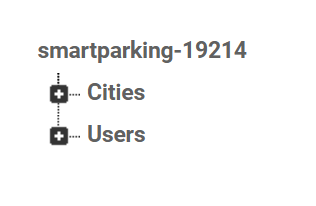
\includegraphics[scale=1]{db_general.png}
\end{figure}

\paragraph{Cities} 
In this folder are stored all the Cities included in the project, and each of them contains all the parking Areas that will be shown to the user. 
\begin{figure}[H]
\centering
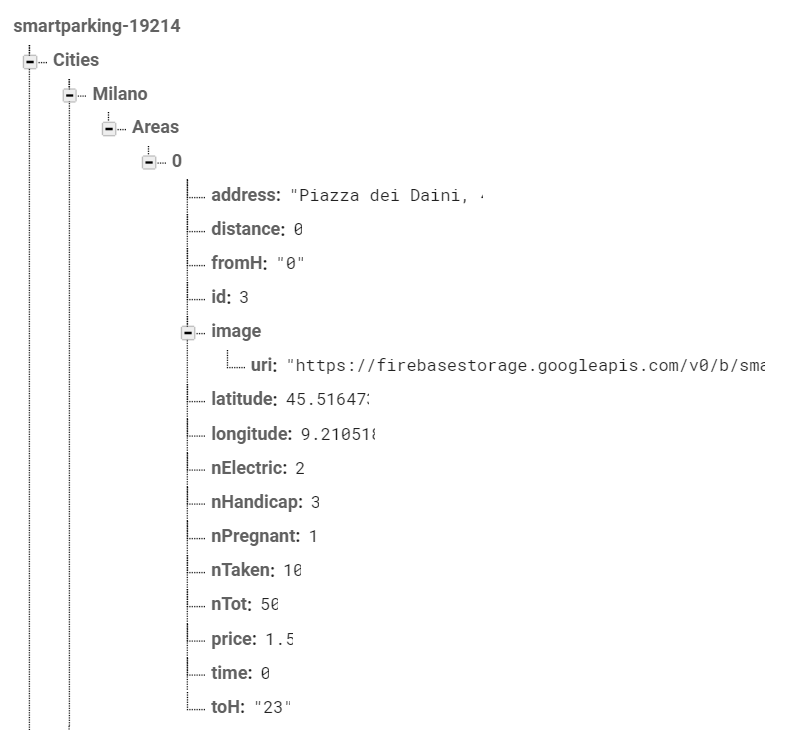
\includegraphics[scale=1]{db_area.png}
\end{figure}


\paragraph{Users} 
In this folder are stored all the Users registered to SmartParking (by their ID), and each of them contains all the needed information about them such as e-mail, name, preferences, etc.. 
\begin{figure}[H]
\centering
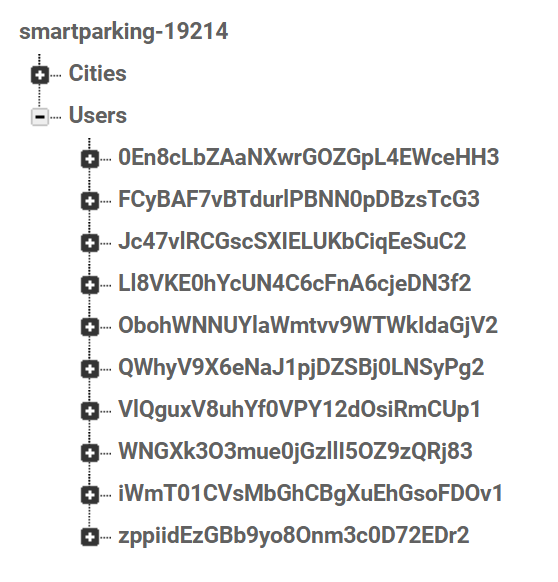
\includegraphics[scale=1]{db_users.png}
\end{figure}

\subsection{Architectural styles and patterns}
\subsubsection{Design Patterns}
\begin{itemize}
\item \texttt{Model-View-Controller Pattern}: is a software design pattern commonly used for developing user interfaces which divides the related program logic into three interconnected elements. This is done to separate internal representations of information from the ways information is presented to and accepted from the user. Following the MVC architectural pattern decouples these major components allowing for code reuse and parallel development. \\In SmartParking, we can say that the \texttt{Mobile App} represents both the \textbf{View} and the \textbf{Controller} of the system, while the entire \texttt{Back end} and in particular the Database represents the \textbf{Model}. That is, the App shows the relevant data to the user, and provide the possibility to choose between some options to modify the shown data: it behaves like a Controller, calling fetch methods to update the Server-side data. \\It is worth to mention that, in some cases, the MVC Pattern with a local copy on the client side has been used: this because relying on fetch methods everytime the user modifies some data would be too heavy from a computational point of view, and also too much internet-consuming.  

\item \texttt{Observer/Observable Pattern}: is used when there is one-to-many relationship between objects such as if one object is modified, its depenedent objects are to be notified automatically. Observer pattern falls under behavioral pattern category. This is the natural Design Pattern used to implement the MVC Pattern: in our system, the intent of this pattern is to let the User execute some queries through the UI and after searching the Database, the result is shown back in the UI. If changes occurs in the database, the UI is notified and updates the UI. \\We can say that React Native helped us a lot in implementing this pattern, due to the intrinsic presence of this. All RN components, in fact, are "linked" to state values, and modifying them results in modifying also the UI to which the value is linked. 
\end{itemize}

\section{Third Party interaction}
\subsection{Google}
\subsection{Facebook}
\subsection{Paypal}
\begin{figure}[H]
\centering
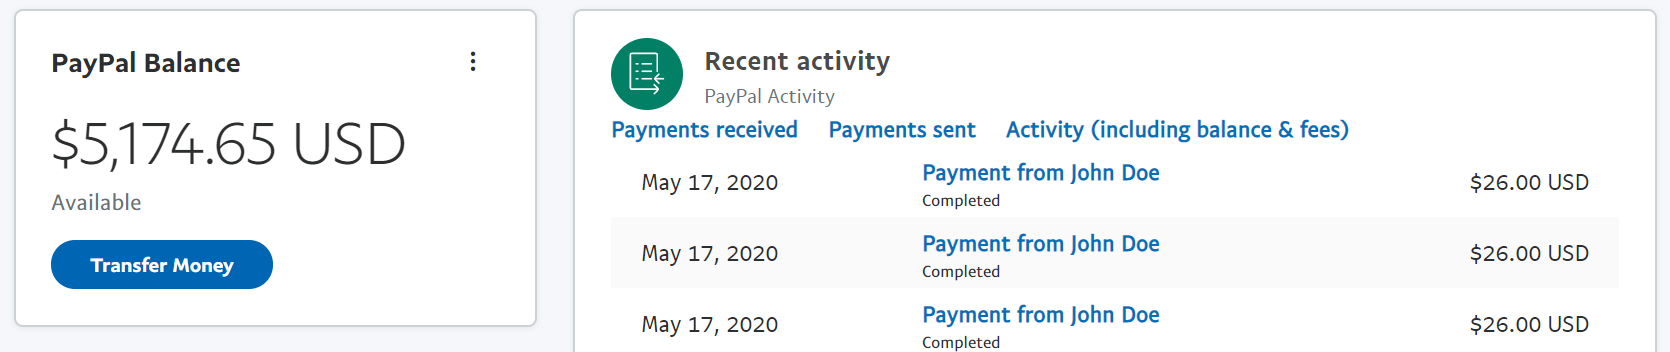
\includegraphics[scale=0.5]{paypal_merchant.png}
\caption{Merchant account history of received payments}
\end{figure}
\begin{figure}[H]
\centering
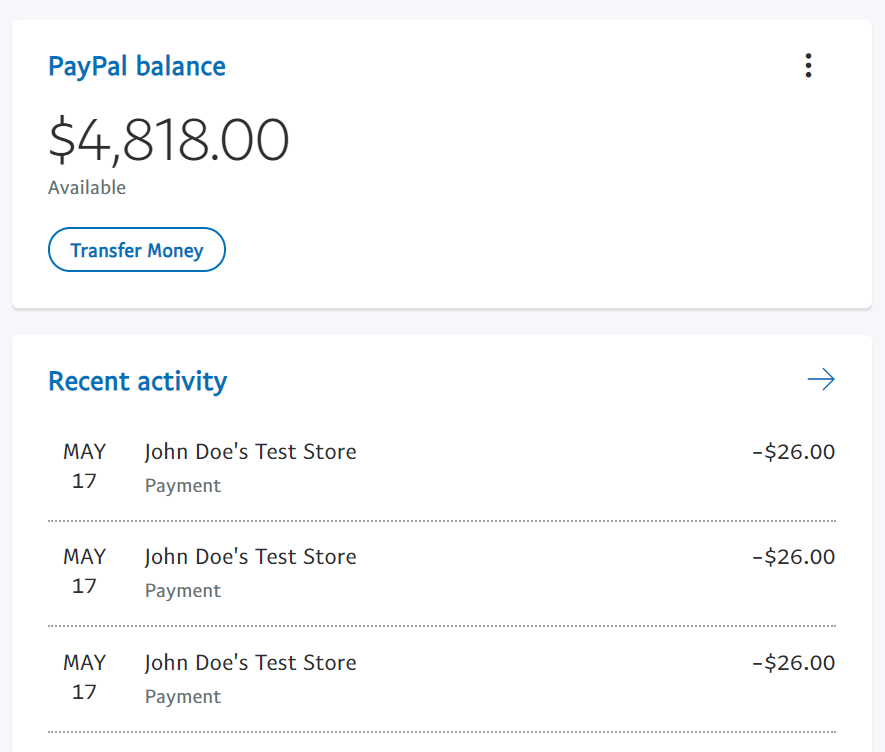
\includegraphics[scale=0.5]{paypal_customer.png}
\caption{Customer account history of processed payments}
\end{figure}
\subsection{Stripe}
\begin{figure}[H]
\centering
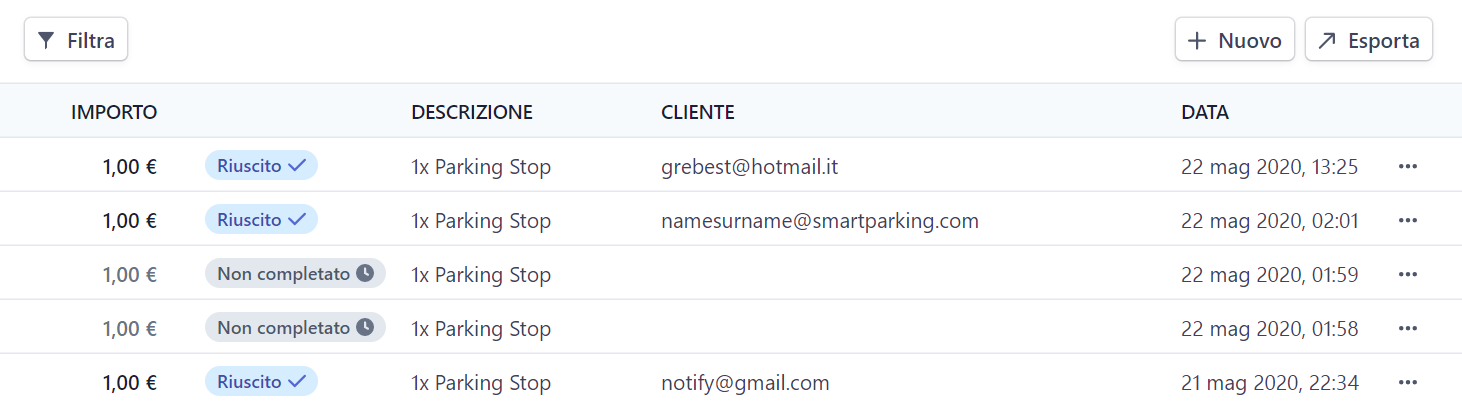
\includegraphics[scale=0.5]{stripe.png}
\caption{History of payments received or deleted by users}
\end{figure}
\subsection{Redux}
\subsection{Google Maps APIs}


\section{User Interface Design}
In this section we will describe, page by page, all the Screens of the Mobile Application and their functionalities, along with the decisions we made to provide a nice and pleasant User Experience.
\subsection{Colors}
\subsection{Fonts}

\subsection{Splash Screen}
\subsection{Welcome Screen}
\subsection{Login Screen}
\subsection{Registration Screen}
\subsection{Home/Map Screen}
\subsection{Parking Screen(s)}
\paragraph{List Screen}
\paragraph{Active Parking Screen}
\paragraph{History Screen}
\subsection{Filter Screen}
\subsection{Profile Screen}

\section{Implementation and Integration}
We can split this section in three main phases, written in order of implementation: 

\subsection{Front End implementation}
First of all we created all the needed screens with a very basic design: we were focused on providing a good User eXperience flow first by identifying all the best components to insert, and only after this phase we started thinking about the color, shape and less-relevant details. This is a very common development flow in mobile applications, and works very well when managing a lot of screens and user flow possibilities.   
\subsection{Back End implementation}
We created the Back end skeleton of the system, by configuring Firebase Realtime Database in order to store every needed information. In particular, we started by organizing and adding all the involved Cities (in the very first version only Milan and Sondrio, the group members' cities), and then adding to them all the parking Areas. 
\subsection{Front End and Back End integration}
This phase was relatively short, because 

\section{Testing}
Nothing.

\end{document}
